%%%%%%%% ICML 2018 EXAMPLE LATEX SUBMISSION FILE %%%%%%%%%%%%%%%%%

\documentclass{article}

% Recommended, but optional, packages for figures and better typesetting:
\usepackage{microtype}
\usepackage{graphicx}
\usepackage{subfigure}
\usepackage{booktabs} % for professional tables

% added packages david
\usepackage{amsmath, amssymb}
\usepackage{bm}
\usepackage{subfigure}
\usepackage{tikz}


% hyperref makes hyperlinks in the resulting PDF.
% If your build breaks (sometimes temporarily if a hyperlink spans a page)
% please comment out the following usepackage line and replace
% \usepackage{icml2018} with \usepackage[nohyperref]{icml2018} above.
\usepackage{hyperref}

% Attempt to make hyperref and algorithmic work together better:
\newcommand{\theHalgorithm}{\arabic{algorithm}}

\newcommand\independent{\protect\mathpalette{\protect\independenT}{\perp}}
\def\independenT#1#2{\mathrel{\rlap{$#1#2$}\mkern2mu{#1#2}}}

% Use the following line for the initial blind version submitted for review:
%\usepackage{icml2018_ift6269}

% If accepted, instead use the following line for the camera-ready submission:
\usepackage[accepted]{icml2018_ift6269}
% SLJ: -> use this for your IFT 6269 project report!

% The \icmltitle you define below is probably too long as a header.
% Therefore, a short form for the running title is supplied here:
\icmltitlerunning{Implementation of a probabilistic Softmax for BNNs}

\begin{document}

\twocolumn[
\icmltitle{Implementation of a probabilistic Softmax for BNNs}

% It is OKAY to include author information, even for blind
% submissions: the style file will automatically remove it for you
% unless you've provided the [accepted] option to the icml2018
% package.

% List of affiliations: The first argument should be a (short)
% identifier you will use later to specify author affiliations
% Academic affiliations should list Department, University, City, Region, Country
% Industry affiliations should list Company, City, Region, Country

% You can specify symbols, otherwise they are numbered in order.
% Ideally, you should not use this facility. Affiliations will be numbered
% in order of appearance and this is the preferred way.
\icmlsetsymbol{equal}{*}

\begin{icmlauthorlist}
\icmlauthor{Aeiau Zzzz}{equal,to}
\icmlauthor{Bauiu C.~Yyyy}{equal,to,goo}
\icmlauthor{Cieua Vvvvv}{goo}
\icmlauthor{Iaesut Saoeu}{ed}
\icmlauthor{Fiuea Rrrr}{to}
\icmlauthor{Tateu H.~Yasehe}{ed,to,goo}
\icmlauthor{Aaoeu Iasoh}{goo}
\icmlauthor{Buiui Eueu}{ed}
\icmlauthor{Aeuia Zzzz}{ed}
\icmlauthor{Bieea C.~Yyyy}{to,goo}
\icmlauthor{Teoau Xxxx}{ed}
\icmlauthor{Eee Pppp}{ed}
\end{icmlauthorlist}

\icmlaffiliation{to}{Department of Computation, University of Torontoland, Torontoland, Canada}
\icmlaffiliation{goo}{Googol ShallowMind, New London, Michigan, USA}
\icmlaffiliation{ed}{School of Computation, University of Edenborrow, Edenborrow, United Kingdom}

\icmlcorrespondingauthor{Cieua Vvvvv}{c.vvvvv@googol.com}
\icmlcorrespondingauthor{Eee Pppp}{ep@eden.co.uk}



% You may provide any keywords that you
% find helpful for describing your paper; these are used to populate
% the "keywords" metadata in the PDF but will not be shown in the document
\icmlkeywords{Machine Learning, ICML}

\vskip 0.3in
]

% this must go after the closing bracket ] following \twocolumn[ ...

% This command actually creates the footnote in the first column
% listing the affiliations and the copyright notice.
% The command takes one argument, which is text to display at the start of the footnote.
% The \icmlEqualContribution command is standard text for equal contribution.
% Remove it (just {}) if you do not need this facility.

%\printAffiliationsAndNotice{}  % leave blank if no need to mention equal contribution
\printAffiliationsAndNotice{\icmlEqualContribution} % otherwise use the standard text.

\begin{abstract}
This document provides a basic paper template and submission guidelines.
Abstracts must be a single paragraph, ideally between 4--6 sentences long.
Gross violations will trigger corrections at the camera-ready phase.
\end{abstract}

\section{Introduction}\label{sec:intro}

In recent years, deep learning has achieved remarkable success across a wide range of classification tasks, including image recognition, natural language processing, and medical diagnosis \cite{lecun2015deep}. Despite their high predictive accuracy, traditional neural networks often operate as black boxes, providing point estimates without quantifying the uncertainty associated with their predictions. This limitation poses significant challenges, especially in safety-critical applications such as autonomous driving, healthcare, and financial decision-making, where understanding the confidence of predictions is crucial for reliable and trustworthy outcomes \cite{kendall2017uncertainties}. Uncertainty estimation in neural networks addresses this challenge by providing measures of confidence alongside predictions. Bayesian Neural Networks (BNNs) offer a principled framework for uncertainty estimation by treating model parameters as random variables and capturing their posterior distribution \cite{blundell15}. By integrating over the uncertainty in the model parameters, BNNs can provide more robust predictions and better generalize to unseen data. However, exact Bayesian inference in neural networks is intractable due to the high dimensionality and complexity of the parameter space, necessitating the development of approximate inference methods. Several approaches have been proposed to approximate the posterior distribution in BNNs, each with its own set of advantages and limitations. Sampling-based methods like Stochastic Gradient Langevin Dynamics (SGLD) \cite{} and Hamiltonian Monte Carlo (HMC) \cite{neal12} provide accurate posterior approximations but are often computationally expensive and challenging to scale to large networks. On the other hand, approximation techniques such as Monte Carlo Dropout (MC Dropout) \cite{gal16} and Deep Ensembles \cite{lakshminarayanan17} offer more computationally feasible alternatives but may lack the theoretical rigor and flexibility to capture complex posterior distributions fully. Variational Inference (VI) methods, including Bayesian Backpropagation (BBP) \cite{blundell15}, strike a balance between scalability and accuracy but are constrained by the choice of variational families, which may oversimplify the true posterior. Despite these advancements, existing methods often face trade-offs between computational efficiency, scalability, and the fidelity of uncertainty estimates. In particular, many approaches rely on assumptions such as Gaussianity in the parameter or output space, which may not hold in practice, especially for complex and high-dimensional data distributions. Additionally, the computational overhead associated with sampling-based methods limits their applicability to large-scale classification tasks, prompting the need for more efficient inference techniques.

In this work, we implement a novel method that leverages Tractable Approximate Gaussian Inference (TAGI) to provide efficient and scalable uncertainty estimation in Bayesian Deep Networks. TAGI offers an to sampling-based approaches by maintaining and updating approximate Gaussian distributions over network parameters, enabling the propagation of uncertainty through deep learning models seamlessly. Furthermore, we propose a probabilistic softmax formulation that translates the uncertainty from the logit space to the output space, allowing for accurate and computationally efficient uncertainty estimates in classification tasks.

The focus of our project can be summarized as follows:

\begin{itemize}
    \item \textbf{Tractable Approximate Gaussian Inference (TAGI):} We re-implement the toy example proposed in the original TAGI paper \cite{goulet2020tractable}.
    \item \textbf{Probabilistic Softmax for Uncertainty Estimation:} We provide an implementation of the probabilistic softmax formulation porposed by the authors of TAGI on C++ and CUDA for the cutagi library \cite{}, along with an evaluation on datasets such as MNIST and CIFAR-10.
    \item \textbf{Ablation Study:} We conduct an ablation study to evaluate the effectiveness of TAGI-based inference and the probabilistic softmax formulation in uncertainty estimation for classification tasks.
\end{itemize}

\section{Related Work}\label{sec:related_work}
Bayesian Neural Networks (BNNs) provide a principled framework for uncertainty estimation by capturing a posterior distribution over model parameters. Various methods, including sampling-based techniques and approximations, have been proposed to estimate uncertainty in classification tasks efficiently. Below, we review prominent methods alongside a recent advance using analytical approximations.

\subsection{Monte Carlo Dropout (MC Dropout)}
MC Dropout, introduced by \cite{gal16}, approximates Bayesian inference by using dropout during both training and inference. Multiple stochastic forward passes are performed at inference by sampling different dropout masks, and the outputs are aggregated to estimate the predictive distribution. The predictive mean is computed as:
$$
\hat{\mathbf{y}} = \frac{1}{T} \sum_{t=1}^{T} f(\mathbf{x}, \mathbf{w}^{(t)}),
$$
where  $\mathbf{w}^{(t)}$  are the sampled weights with dropout and  $T$  is the number of stochastic passes. This approach is computationally efficient and easy to implement but is limited by the reliance on dropout regularization, which might not fully capture posterior uncertainty.

\subsection{Stochastic Gradient Langevin Dynamics (SGLD)}
SGLD, proposed by \cite{well11}, combines stochastic gradient descent (SGD) with Langevin dynamics to sample from the posterior distribution of weights. The weight updates include Gaussian noise:
$$
\mathbf{w}_{t+1} = \mathbf{w}_t - \eta \nabla \mathcal{L}(\mathbf{w}_t) + \sqrt{2\eta} \epsilon_t,
$$
where  $\eta$  is the learning rate,  $\mathcal{L}$  is the loss function, and  $\epsilon_t \sim \mathcal{N}(0, I)$  is Gaussian noise. By incorporating noise into the gradient updates, SGLD provides samples that approximate the posterior. However, the method is more computationally intensive compared to approximation techniques like MC Dropout and can be sensitive to hyperparameters such as the step size.

\subsection{Hamiltonian Monte Carlo (HMC)}
HMC \cite{neal12} extends traditional Markov Chain Monte Carlo (MCMC) by using Hamiltonian dynamics to sample efficiently from the posterior. It introduces momentum variables and explores the posterior landscape using the Hamiltonian:
$$
\mathcal{H}(\mathbf{w}, \mathbf{p}) = -\log p(\mathbf{w} | \mathcal{D}) + \frac{\|\mathbf{p}\|^2}{2},
$$
where  $\mathbf{p}$  is the momentum. HMC provides accurate posterior samples, but its computational cost is prohibitive for high-dimensional neural network parameters. Additionally, it requires careful tuning of the step size and number of leapfrog steps.

\subsection{Bayesian Backpropagation (BBP)}
Bayesian Backpropagation (BBP), also known as Bayes by Backprop \cite{blundell15}, uses variational inference to approximate the posterior distribution over weights. A variational distribution  $q(\mathbf{w})$ , typically Gaussian, is optimized to minimize the Kullback-Leibler (KL) divergence from the true posterior. The variational posterior is parameterized as:
$$
q(\mathbf{w} | \boldsymbol{\theta}) = \prod_{i} \mathcal{N}(w_i; \mu_i, \sigma_i^2),
$$
where  $\boldsymbol{\theta} = (\boldsymbol{\mu}, \boldsymbol{\sigma})$  are learnable parameters. Inference involves sampling weights from  $q(\mathbf{w})$  and averaging multiple forward passes. While BBP provides a principled approach to Bayesian inference, the quality of the approximation depends on the chosen variational family, which might not fully capture the true posterior.

\subsection{Deep Ensembles}
Deep Ensembles \cite{NIPS2017} estimate uncertainty by training multiple neural networks with different random initializations. The ensemble predictions are averaged to compute the predictive distribution:
$$
\hat{\mathbf{y}} = \frac{1}{M} \sum_{m=1}^{M} f(\mathbf{x}; \mathbf{w}_m),
$$
where  $\mathbf{w}_m$  are the weights of the  $m^{th}$ ensemble member. The variance across the ensemble outputs represents model uncertainty. This method is robust and often outperforms other techniques in practice. However, it is computationally expensive due to the need to train multiple models independently.

\subsection{Variational Inference (VI)}
Variational Inference \cite{NIPS2011} approximates the posterior distribution  $p(\mathbf{w} | \mathcal{D})$  with a simpler variational distribution  $q(\mathbf{w})$  by minimizing the KL divergence:
$$
\text{KL}(q(\mathbf{w}) \| p(\mathbf{w} | \mathcal{D})) = \int q(\mathbf{w}) \log \frac{q(\mathbf{w})}{p(\mathbf{w} | \mathcal{D})} \, d\mathbf{w}.
$$
Common variational families include mean-field Gaussians, which are computationally efficient but may not fully capture the complexity of the true posterior. Variational inference is scalable and adaptable but often trades accuracy for efficiency.

\subsection{Fast Predictive Uncertainty for Classification with Bayesian Deep Networks}
\cite{hobbhahn22a} propose a method that revisits the Laplace Bridge technique to approximate the softmax output distribution using a Dirichlet distribution. The method maps Gaussian distributions in logit space  $\mathcal{N}(\mu, \Sigma)$  to Dirichlet distributions in output space  $\text{Dir}(\boldsymbol{\alpha})$  via the analytical mapping:
$$
\alpha_k = \exp\left(\mu_k + \frac{\sigma_k^2}{2}\right), \quad \text{for } k = 1, \ldots, K,
$$
where  $\mu_k$  and  $\sigma_k^2$  are the mean and variance of the logit for class  $k$ , and  $\alpha_k$  is the parameter of the resulting Dirichlet distribution. This approach avoids sampling and significantly reduces computational costs. It scales effectively to large datasets like ImageNet and complex architectures like DenseNet. While the method is efficient, its limitations include reliance on Gaussian assumptions in logit space and potential inaccuracies in modeling highly non-Gaussian posteriors. Additionally, its performance on small or imbalanced datasets is underexplored.

Each method offers unique strengths and weaknesses. MC Dropout and Deep Ensembles are practical and straightforward but may lack the theoretical rigor of sampling-based methods like SGLD and HMC. Variational inference approaches, such as BBP, balance scalability and accuracy but depend heavily on the choice of variational family. Sampling-based methods like SGLD and HMC provide accurate posterior approximations but are computationally expensive. The Dirichlet-based approach by Hobbhahn et al. introduces computational efficiency and scalability but trades off some flexibility in capturing complex posterior distributions.

In the next section, we introduce a novel method that combines the efficiency of analytical approximations with the theoretical grounding of Bayesian inference. The method relies on Tractable Approximate Gaussian Inference (TAGI) as a learning paradigm that allows passing uncertainty through deep learning models, and the formulation of a probabilistic softmax that further allows passing that uncertainty to the output layer.

\section{Methodology}\label{sec:methodology}
\subsection{Tractable approximate gaussian inference (TAGI)}\label{sub:tagi}
Goulet et al. \cite{goulet2020tractable} proposed the Tractable Approximate Gaussian Inference (TAGI) method, which is a Bayesian approach to neural networks. Compared to traditional NNs, this method allows to (1) optimize parameters analytically, (2) treat uncertainties from input to output layers and provide density forecasts. \\
Consider a fully connected NN presented in Figure \ref{fig:FNN},
the formulations of a TAGI-NN, which is similar to that of a traditional NN except that parameters and variables are assumed to be normally distributed, are defined by the following deterministic equations:
\begin{equation*} \label{eq:TAGI}
\begin{split}
    \bm{z}^{(1)} &= \bm{w}^{(0)} \bm{x} + \bm{b}^{(0)}, \\
    \bm{a}^{(i)} &= \tilde{\sigma}(\bm{z}^{(i)}) \; \; \;(i=1:\mathtt{L}), \\
    \bm{z}^{(i)} &= \bm{w}^{(i)} \bm{a}^{(i-1)} + \bm{b}^{(i)} \; \; \;(i=2:\mathtt{L}), \\
    \bm{z}^{(\mathtt{O})} &=  \bm{w}^{(\mathtt{L})} \bm{a}^{(\mathtt{L})} + \bm{w}^{(\mathtt{L})} \\
    \bm{y} &=  \bm{z}^{(\mathtt{O})} + \bm{v}.
\end{split}
\end{equation*}
where $\bm{w},\bm{b}$ are parameters, $\mathtt{L}$ is the number of hidden layers, $\bm{v}$ are the observation noise, $\bm{z}$ are hidden units, $\bm{y}$ are outputs, and $\tilde{\sigma}(\cdot)$ is the linearized activation function.
\begin{figure}[htbp]
\centering
\subfigure[]{\resizebox{0.9\linewidth}{!}{
\tikzset{dist1/.style={path picture= {
    \begin{scope}[x=1pt,y=10pt]
      \draw plot[domain=-6:6] (\x,{1/(1 + exp(-\x))-0.5});
    \end{scope}
    }
  }
}
\tikzset{dist2/.style={path picture= {
    \begin{scope}[x=1pt,y=10pt]
      \draw plot[domain=-6:6] (\x,{\x/10});
    \end{scope}
    }
  }
}
\tikzstyle{input}=[draw,fill=red!10,circle,minimum size=15pt,inner sep=0pt]
\tikzstyle{hidden}=[draw,fill=green!20,circle,minimum size=15pt,inner sep=0pt]
\tikzstyle{output}=[draw,fill=blue!20,circle,minimum size=15pt,inner sep=0pt]
\tikzstyle{bias}=[draw=none,circle,minimum size=15pt,inner sep=0pt]


\tikzstyle{stateTransition}=[->,line width=0.25pt,draw=black!50]


\begin{tikzpicture}[scale=1.36]\scriptsize
    \node (x1)[input]   at (0, 1.25) {$x_{1}$};
    \node (x2)[input] at (0, 0.25) {$x_{2}$};
    \node (x3)  at (0,-0.5) {\raisebox{6pt}{\vdots}};
    \node (xx)[input]  at (0,-1.25) {$x_{\mathtt{X}}$};

    \node (b0)[bias]  at (0.35,1.9) {$\bm{b}^{(0)}$};


    \node (h11)[hidden] at (1, 1.5) {$z^{(1)}_{1}$};
    \node (h12)[hidden] at (1, 0.5) {$z^{(1)}_{2}$};
    \node (h13) at (1,-0.5) {\raisebox{5pt}{$\vdots$}};
    \node (h14)[hidden] at (1,-1.5) {$z^{(1)}_{\mathtt{A}}$};
    \node (b1)[bias]  at (1.35,1.9) {$\bm{b}^{(1)}$};

    \node (h21)[hidden] at (2, 1.5) {$z^{(2)}_{1}$};
    \node (h22)[hidden] at (2, 0.5) {$z^{(2)}_{2}$};
    \node (h23) at (2,-0.5) {\raisebox{6pt}{\vdots}};
    \node (h24)[hidden] at (2,-1.5) {$z^{(2)}_{\mathtt{A}}$};
    \node (b2)[bias]  at (2.35,1.9) {$\bm{b}^{(\cdots)}$};
    
    \node (h31) at (3, 1.5) {$\cdots$};
    \node (h32) at (3, 0.5) {$\cdots$};
    \node (h33) at (3,-0.5) {\raisebox{6pt}{\vdots}};
    \node (h34) at (3,-1.5) {$\cdots$};
    \node (b3)[bias]  at (3.35,1.9) {$\bm{b}^{(\mathtt{L}-1)}$};
    
    \node (h41)[hidden] at (4, 1.5) {$z^{(\mathtt{L})}_{1}$};
    \node (h42)[hidden] at (4, 0.5) {$z^{(\mathtt{L})}_{2}$};
    \node (h43) at (4,-0.5) {\raisebox{6pt}{\vdots}};
    \node (h44)[hidden] at (4,-1.5) {$z^{(\mathtt{L})}_{\mathtt{A}}$};
    \node (b4)[bias]  at (4.35,1.9) {$\bm{b}^{(\mathtt{L})}$};

    \node (h1)[hidden] at (5.1,1.25) {$z_{1}^{(\mathtt{O})}$};
    \node (h2)[hidden] at (5.1,0.25) {$z_{2}^{(\mathtt{O})}$};
    \node (hn) at (5.1,-0.5) {\raisebox{6pt}{\vdots}};
    \node (h3)[hidden] at (5.1,-1.25) {$z_{\mathtt{Y}}^{(\mathtt{O})}$};
    \node (o1)[output] at (5.7,1.25) {$y_{1}$};
    \node (o2)[output] at (5.7,0.25) {$y_{2}$};
    \node (on) at (5.7,-0.5) {\raisebox{6pt}{\vdots}};
    \node (o3)[output] at (5.7,-1.25) {$y_{\mathtt{Y}}$};
    

    \draw[stateTransition] (x1) -- (h11) node  {};
    \draw[stateTransition] (x1) -- (h12) node  {};
    \draw[stateTransition] (x1) -- (h13) node  {};
    \draw[stateTransition] (x1) -- (h14) node  {};
    \draw[stateTransition] (x2) -- (h11) node  {};
    \draw[stateTransition] (x2) -- (h12) node  {};
    \draw[stateTransition] (x2) -- (h13) node  {};
    \draw[stateTransition] (x2) -- (h14) node  {};
    \draw[stateTransition] (x3) -- (h11) node  {};
    \draw[stateTransition] (x3) -- (h12) node  {};
    \draw[stateTransition] (x3) -- (h13) node  {};
    \draw[stateTransition] (x3) -- (h11) node  {};
    \draw[stateTransition] (xx) -- (h11) node  {};
    \draw[stateTransition] (xx) -- (h12) node  {};
    \draw[stateTransition] (xx) -- (h13) node  {};
    \draw[stateTransition] (xx) -- (h11) node  {};
     \draw[stateTransition] (xx) -- (h14) node  {};
    
    \draw[stateTransition] (b0) -- (h12) node {};
    \draw[stateTransition] (b0) -- (h11) node {};
    \draw[stateTransition] (b0) -- (h13) node {};
    \draw[stateTransition] (b0) -- (h14) node {};

    \draw[stateTransition,opacity=1] (h11) -- (h21) node [midway, rotate=0,fill=white,opacity=0.8] {\scriptsize$w^{(1)}_{1,1}$};
    \draw[stateTransition,opacity=0] (h11) -- (h21) node [midway, rotate=0,fill=white] {\scriptsize$w^{(1)}_{1,1}$};
    \draw[stateTransition,opacity=0.2] (h11) -- (h22) node  {};
    \draw[stateTransition,opacity=0.2] (h11) -- (h23) node  {};
    \draw[stateTransition,opacity=0.2] (h11) -- (h24) node  {};
    \draw[stateTransition,opacity=1] (h12) -- (h21) node [midway, rotate=45,fill=white,opacity=0.8] {\scriptsize$w^{(1)}_{1,2}$};
        \draw[stateTransition,opacity=0] (h12) -- (h21) node [midway, rotate=45,fill=white!90] {\scriptsize$w^{(1)}_{2,1}$};
    \draw[stateTransition,opacity=0.2] (h12) -- (h22) node  {};
    \draw[stateTransition,opacity=0.2] (h12) -- (h23) node  {};
    \draw[stateTransition,opacity=0.2] (h12) -- (h24) node  {};
    %\draw[stateTransition,opacity=0.2] (h13) -- (h21) node  {};
        \draw[stateTransition,opacity=1] (h13) -- (h21) node [midway, rotate=60,fill=white,opacity=0.8] {\scriptsize$w^{(1)}_{1,i}$};
     \draw[stateTransition,opacity=0] (h13) -- (h21) node [midway, rotate=60] {\scriptsize$w^{(1)}_{i,1}$};
    \draw[stateTransition,opacity=0.2] (h13) -- (h22) node  {};
    \draw[stateTransition,opacity=0.2] (h13) -- (h23) node  {};
    \draw[stateTransition,opacity=0.2] (h13) -- (h24) node  {};
    \draw[stateTransition,opacity=1] (h14) -- (h21) node [midway, rotate=70,fill=white,opacity=0.8] {\scriptsize$w^{(1)}_{1,\mathtt{A}}$};
     \draw[stateTransition,opacity=0] (h14) -- (h21) node [midway, rotate=70] {\scriptsize$w^{(1)}_{\mathtt{A},1}$};
    \draw[stateTransition,opacity=0.2] (h14) -- (h22) node  {};
    \draw[stateTransition,opacity=0.2] (h14) -- (h23) node  {};
    \draw[stateTransition,opacity=0.2] (h14) -- (h24) node  {};

    
    \draw[stateTransition,opacity=1] (b1) -- (h21) node  [midway,above=-0.05cm, rotate=-25] {\scriptsize$b^{(1)}_{1}$};
    \draw[stateTransition,opacity=0.2] (b1) -- (h22) node {};
    \draw[stateTransition,opacity=0.2] (b1) -- (h23) node {};
    \draw[stateTransition,opacity=0.2] (b1) -- (h24) node {};
    
     \draw[stateTransition] (h21) -- (h31) node  {};
    \draw[stateTransition] (h21) -- (h32) node  {};
    \draw[stateTransition] (h21) -- (h33) node  {};
    \draw[stateTransition] (h21) -- (h34) node  {};
    \draw[stateTransition] (h22) -- (h31) node  {};
    \draw[stateTransition] (h22) -- (h32) node  {};
    \draw[stateTransition] (h22) -- (h33) node  {};
    \draw[stateTransition] (h22) -- (h34) node  {};
    \draw[stateTransition] (h23) -- (h31) node  {};
    \draw[stateTransition] (h23) -- (h32) node  {};
    \draw[stateTransition] (h23) -- (h33) node  {};
    \draw[stateTransition] (h23) -- (h34) node  {};
    \draw[stateTransition] (h24) -- (h31) node  {};
    \draw[stateTransition] (h24) -- (h32) node  {};
    \draw[stateTransition] (h24) -- (h33) node  {};
    \draw[stateTransition] (h24) -- (h31) node  {};
    \draw[stateTransition] (h24) -- (h34) node  {};

    
    \draw[stateTransition] (b2) -- (h32) node {};
    \draw[stateTransition] (b2) -- (h31) node {};
    \draw[stateTransition] (b2) -- (h33) node {};
    \draw[stateTransition] (b2) -- (h34) node {};
    
    \draw[stateTransition] (h31) -- (h41) node  {};
    \draw[stateTransition] (h31) -- (h42) node  {};
    \draw[stateTransition] (h31) -- (h43) node  {};
    \draw[stateTransition] (h31) -- (h44) node  {};
    \draw[stateTransition] (h32) -- (h41) node  {};
    \draw[stateTransition] (h32) -- (h42) node  {};
    \draw[stateTransition] (h32) -- (h43) node  {};
    \draw[stateTransition] (h32) -- (h44) node  {};
    \draw[stateTransition] (h33) -- (h41) node  {};
    \draw[stateTransition] (h33) -- (h42) node  {};
    \draw[stateTransition] (h33) -- (h43) node  {};
    \draw[stateTransition] (h33) -- (h44) node  {};
    \draw[stateTransition] (h34) -- (h41) node  {};
    \draw[stateTransition] (h34) -- (h42) node  {};
    \draw[stateTransition] (h34) -- (h43) node  {};
    \draw[stateTransition] (h34) -- (h41) node  {};
     \draw[stateTransition] (h34) -- (h44) node  {};
    
    \draw[stateTransition] (b3) -- (h42) node {};
    \draw[stateTransition] (b3) -- (h41) node {};
    \draw[stateTransition] (b3) -- (h43) node {};
    \draw[stateTransition] (b3) -- (h44) node {};
    
    
    \draw[stateTransition] (h41) -- (h1) node  {};
    \draw[stateTransition] (h42) -- (h1) node  {};
    \draw[stateTransition] (h43) -- (h1) node  {};
    \draw[stateTransition] (h44) -- (h1) node  {};
    \draw[stateTransition] (b4) -- (h1) node {};
    
    \draw[stateTransition] (h41) -- (h2) node  {};
    \draw[stateTransition] (h42) -- (h2) node  {};
    \draw[stateTransition] (h43) -- (h2) node  {};
    \draw[stateTransition] (h44) -- (h2) node  {};
    \draw[stateTransition] (b4) -- (h2) node {};
    
    \draw[stateTransition] (h41) -- (hn) node  {};
    \draw[stateTransition] (h42) -- (hn) node  {};
    \draw[stateTransition] (h43) -- (hn) node  {};
    \draw[stateTransition] (h44) -- (hn) node  {};
    \draw[stateTransition] (b4) -- (hn) node {};
    
    \draw[stateTransition] (h41) -- (h3) node  {};
    \draw[stateTransition] (h42) -- (h3) node  {};
    \draw[stateTransition] (h43) -- (h3) node  {};
    \draw[stateTransition] (h44) -- (h3) node  {};
    \draw[stateTransition] (b4) -- (h3) node {};
    
     \draw[stateTransition] (h1) -- (o1) node  {};
     \draw[stateTransition] (h2) -- (o2) node  {};
     \draw[stateTransition] (hn) -- (on) node  {};
     \draw[stateTransition] (h3) -- (o3) node  {};
     
     \node (h12)[hidden] at (1, 0.5) {$z^{(1)}_{2}$};
     \node (h22)[hidden] at (2, 0.5) {$z^{(2)}_{2}$};

\end{tikzpicture}
}}\\
\subfigure[]{\resizebox{0.9
\linewidth}{!}{
\tikzset{dist1/.style={path picture= {
    \begin{scope}[x=1pt,y=10pt]
      \draw plot[domain=-6:6] (\x,{1/(1 + exp(-\x))-0.5});
    \end{scope}
    }
  }
}
\tikzset{dist2/.style={path picture= {
    \begin{scope}[x=1pt,y=10pt]
      \draw plot[domain=-6:6] (\x,{\x/10});
    \end{scope}
    }
  }
}
\tikzstyle{input}=[draw,fill=red!10,circle,minimum size=15pt,inner sep=0pt]
\tikzstyle{hidden}=[draw,fill=green!20,circle,minimum size=15pt,inner sep=0pt]
\tikzstyle{output}=[draw,fill=blue!20,circle,minimum size=15pt,inner sep=0pt]
\tikzstyle{bias}=[draw=none,circle,minimum size=15pt,inner sep=0pt]


\tikzstyle{stateTransition}=[->,line width=0.25pt,draw=black!50]


\begin{tikzpicture}[scale=1.36]\scriptsize
    \node (x)[input]   at (0, 1.5) {$\bm{x}$};
    \node (z1)[hidden] at (1, 1.5) {$\,\bm{z}^{(1)}$};
    \node (z2)[hidden] at (2, 1.5) {$\,\bm{z}^{(2)}$};
    \node (zi) at (3, 1.5) {$\cdots$};
    \node (zL)[hidden] at (4, 1.5) {$\,\bm{z}^{(\mathtt{L})}$};
    \node (zO)[hidden] at (5.1,1.5) {$\,\bm{z}^{(\mathtt{O})}$};
        %\node (zO)[hidden,fill=cyan!20] at (5.1,1.5) {$\,\bm{z}^{\!(\mathtt{O})}$};

    \node (y)[output] at (5.7,1.5) {$\bm{y}$};
   
   
    \draw[stateTransition,opacity=1] (x) -- (z1) node [midway, rotate=0,fill=white,opacity=0.8] {\scriptsize$\!\bm{\theta}^{(0)}\!$};
    \draw[stateTransition,opacity=1] (z1) -- (z2) node [midway, rotate=0,fill=white,opacity=0.8] {\scriptsize$\!\bm{\theta}^{(1)}\!$};
     \draw[stateTransition,opacity=1] (z2) -- (zi) node [midway, rotate=0,fill=white,opacity=0.8] {\scriptsize$\!\bm{\theta}^{(2)}\!$};
     \draw[stateTransition,opacity=1] (zi) -- (zL) node [midway, rotate=0,fill=white,opacity=0.8] {\scriptsize$\!\!\bm{\theta}^{(\mathtt{L}\text{-}1)}\!\!$};
    \draw[stateTransition,opacity=1] (zL) -- (zO) node [midway, rotate=0,fill=white,opacity=0.8] {\scriptsize$\!\bm{\theta}^{(\mathtt{L})}\!$};
     \draw[stateTransition,opacity=1] (zO) -- (y);
\end{tikzpicture}
}}
\caption{(a) A neural network representation. (b) A compacted NN representation, reproduced from \cite{goulet2020tractable}.}
\label{fig:FNN}
\end{figure}

In Equation \ref{eq:TAGI}, the product of two Gaussian random variables is not Gaussian, despite of this, the authors proposed using the \textit{Gaussian Multiplication Approximation} (GMA) to approximate the PDF of any product term $X_iX_j$ given by
%

% First Equation
\begin{equation*}
    \mathbb{E}\left[X_{1} X_{2}\right] = \mu_{1} \mu_{2} + \operatorname{cov}\left(X_{1}, X_{2}\right)
\end{equation*}
% Second Equation
\begin{equation*}
    \operatorname{cov}\left(X_{3}, X_{1} X_{2}\right) = \operatorname{cov}\left(X_{1}, X_{3}\right) \mu_{2} + \operatorname{cov}\left(X_{2}, X_{3}\right) \mu_{1}
\end{equation*}
% Third Equation - Split into Multiple Lines
\begin{align*}
    \operatorname{cov}\left(X_{1} X_{2}, X_{3} X_{4}\right) &= \operatorname{cov}\left(X_{1}, X_{3}\right) \operatorname{cov}\left(X_{2}, X_{4}\right) \nonumber \\
    &\quad + \operatorname{cov}\left(X_{1}, X_{4}\right) \operatorname{cov}\left(X_{2}, X_{3}\right) \nonumber \\
    &\quad + \operatorname{cov}\left(X_{1}, X_{3}\right) \mu_{2} \mu_{4} \nonumber \\
    &\quad + \operatorname{cov}\left(X_{1}, X_{4}\right) \mu_{2} \mu_{3} \nonumber \\
    &\quad + \operatorname{cov}\left(X_{2}, X_{3}\right) \mu_{1} \mu_{4} \nonumber \\
    &\quad + \operatorname{cov}\left(X_{2}, X_{4}\right) \mu_{1} \mu_{3}
\end{align*}
% Fourth Equation - Split into Multiple Lines
\begin{align*}
    \operatorname{var}\left(X_{1} X_{2}\right) &= \sigma_{1}^{2} \sigma_{2}^{2} + \operatorname{cov}\left(X_{1}, X_{2}\right)^{2} \nonumber \\
    &\quad + 2 \operatorname{cov}\left(X_{1}, X_{2}\right) \mu_{1} \mu_{2} \nonumber \\
    &\quad + \sigma_{1}^{2} \mu_{2}^{2} + \sigma_{2}^{2} \mu_{1}^{2}
\end{align*}
where $\mu, \sigma$ are respectively the mean and standard deviation of a random variable. 
Unlike a traditional NN where parameters are updated using backpropagation, model parameters in a TAGI-NN can be obtained analytically by a layer-wise scheme as depicted in Figure \ref{fig:updateTAGI}.
\begin{figure}[htbp]
\centering
\resizebox{0.9\linewidth}{!}{
\tikzset{dist1/.style={path picture= {
    \begin{scope}[x=1pt,y=10pt]
      \draw plot[domain=-6:6] (\x,{1/(1 + exp(-\x))-0.5});
    \end{scope}
    }
  }
}
\tikzset{dist2/.style={path picture= {
    \begin{scope}[x=1pt,y=10pt]
      \draw plot[domain=-6:6] (\x,{\x/10});
    \end{scope}
    }
  }
}
\tikzstyle{input}=[draw,fill=red!10,circle,minimum size=15pt,inner sep=0pt]
\tikzstyle{hidden}=[draw,fill=green!20,circle,minimum size=15pt,inner sep=0pt]
\tikzstyle{output}=[draw,fill=blue!20,circle,minimum size=15pt,inner sep=0pt]
\tikzstyle{bias}=[draw=none,circle,minimum size=15pt,inner sep=0pt]


\tikzstyle{stateTransition}=[->,line width=0.25pt,draw=black!50]


\begin{tikzpicture}[scale=1.36]\scriptsize
    \node (x)[input]   at (0, 1.5) {$\bm{x}$};
    \node (z1)[hidden] at (1, 1.5) {$\,\bm{z}^{(1)}$};
    \node (z2)[hidden] at (2, 1.5) {$\,\bm{z}^{(2)}$};
    \node (zi) at (3, 1.5) {$\cdots$};
    \node (zL)[hidden] at (4, 1.5) {$\,\bm{z}^{(\mathtt{L})}$};
    \node (zO)[hidden] at (5.1,1.5) {$\,\bm{z}^{(\mathtt{O})}$};
        %\node (zO)[hidden,fill=cyan!20] at (5.1,1.5) {$\,\bm{z}^{\!(\mathtt{O})}$};

    \node (y)[output] at (5.7,1.5) {$\bm{y}$};
   
   
    \draw[stateTransition,opacity=1] (x) -- (z1) node [midway, rotate=0,fill=white,opacity=0.8] {\scriptsize$\!\bm{\theta}^{(0)}\!$};
    \draw[stateTransition,opacity=1] (z1) -- (z2) node [midway, rotate=0,fill=white,opacity=0.8] {\scriptsize$\!\bm{\theta}^{(1)}\!$};
     \draw[stateTransition,opacity=1] (z2) -- (zi) node [midway, rotate=0,fill=white,opacity=0.8] {\scriptsize$\!\bm{\theta}^{(2)}\!$};
     \draw[stateTransition,opacity=1] (zi) -- (zL) node [midway, rotate=0,fill=white,opacity=0.8] {\scriptsize$\!\!\bm{\theta}^{(\mathtt{L}\text{-}1)}\!\!$};
    \draw[stateTransition,opacity=1] (zL) -- (zO) node [midway, rotate=0,fill=white,opacity=0.8] {\scriptsize$\!\bm{\theta}^{(\mathtt{L})}\!$};
     \draw[stateTransition,opacity=1] (zO) -- (y);
     
     \path (y) edge [->, cyan, opacity=0.8, bend left] (zO);
     \path (zO) edge [->, cyan, opacity=0.8, bend left] (zL);
     \path (zO) edge [->, cyan, opacity=0.8, bend left] (4.5,1.45);
     \path (zL) edge [->, cyan, opacity=0.8, bend left] (3,1.45);
     \path (zL) edge [->, cyan, opacity=0.8, bend left] (3.5,1.45);
     \path (zi) edge [->, cyan, opacity=0.8, bend left] (z2);
     \path (zi) edge [->, cyan, opacity=0.8, bend left] (2.5,1.45);
     \path (z2) edge [->, cyan, opacity=0.8, bend left] (z1);
     \path (z2) edge [->, cyan, opacity=0.8, bend left] (1.5,1.45);
     \path (z1) edge [->, cyan, opacity=0.8, bend left] (.5,1.45);
     
\end{tikzpicture}
}
\caption{Recursive layer-wise inference, reproduced from \cite{goulet2020tractable}.  Cyan arrows indicate inference directions.}
\label{fig:updateTAGI}
\end{figure}
%
First, given the observations $\bm{y}$, the output layer is updated as
\begin{equation*} \label{eq:z0update}
\begin{aligned}
f\left(\boldsymbol{z}^{(\mathtt{O})} \mid \boldsymbol{y}\right) &=\mathcal{N}\left(\boldsymbol{z}^{(\mathtt{O})} ; \boldsymbol{\mu}_{\boldsymbol{Z}^{(\mathtt{O})} \mid \boldsymbol{y}}, \boldsymbol{\Sigma}_{\boldsymbol{Z}^{(\mathtt{O})} \mid \boldsymbol{y}}\right) \\
\boldsymbol{\mu}_{\boldsymbol{Z}^{(\mathtt{O})} \mid \boldsymbol{y}} &=\boldsymbol{\mu}_{\boldsymbol{Z}^{(\mathtt{O})}}+\boldsymbol{\Sigma}_{\boldsymbol{Y} \boldsymbol{Z}^{(\mathtt{O})}}^{\top} \boldsymbol{\Sigma}_{\boldsymbol{Y}}^{-1}\left(\boldsymbol{y}-\boldsymbol{\mu}_{\boldsymbol{Y}}\right) \\
\boldsymbol{\Sigma}_{\boldsymbol{Z}^{(\mathtt{O})} \mid \boldsymbol{y}} &=\boldsymbol{\Sigma}_{\boldsymbol{Z}^{(\mathtt{O})}}-\boldsymbol{\Sigma}_{\boldsymbol{Y} \boldsymbol{Z}^{(\mathtt{O})}}^{\top} \boldsymbol{\Sigma}_{\boldsymbol{Y}}^{-1} \boldsymbol{\Sigma}_{\boldsymbol{Y Z}^{(\mathtt{O})}}.
\end{aligned}
\end{equation*}
%
Next, the hidden units and parameters of the layer $i^{th}$ are updated using a layer-wise procedure as
\begin{equation*}  \label{eq:layerwiseupdate}
\begin{aligned}
f(\boldsymbol{z} \mid \boldsymbol{y}) &=\mathcal{N}\left(\boldsymbol{z} ; \boldsymbol{\mu}_{\boldsymbol{Z} \mid \boldsymbol{y}}, \boldsymbol{\Sigma}_{\boldsymbol{Z} \mid \boldsymbol{y}}\right) \\
\boldsymbol{\mu}_{\boldsymbol{Z} \mid \boldsymbol{y}} &=\boldsymbol{\mu}_{\boldsymbol{Z}}+\mathbf{J}_{\boldsymbol{Z}}\left(\boldsymbol{\mu}_{\boldsymbol{Z}^{+} \mid \boldsymbol{y}}-\boldsymbol{\mu}_{\boldsymbol{Z}^{+}}\right) \\
\boldsymbol{\Sigma}_{\boldsymbol{Z} \mid \boldsymbol{y}} &=\boldsymbol{\Sigma}_{\boldsymbol{Z}}+\mathbf{J}_{\boldsymbol{Z}}\left(\boldsymbol{\Sigma}_{\boldsymbol{Z}^{+} \mid \boldsymbol{y}}-\boldsymbol{\Sigma}_{\boldsymbol{Z}^{+}}\right) \mathbf{J}_{\boldsymbol{Z}}^{\top} \\
\mathbf{J}_{\boldsymbol{Z}} &=\boldsymbol{\Sigma}_{\boldsymbol{Z Z}^{+}} \boldsymbol{\Sigma}_{\boldsymbol{Z}^{+}}^{-1},
\end{aligned}
\end{equation*}
%
\begin{equation*}
\begin{aligned}
f(\boldsymbol{\theta} \mid \boldsymbol{y}) &=\mathcal{N}\left(\boldsymbol{\theta} ; \boldsymbol{\mu}_{\boldsymbol{\theta} \mid \boldsymbol{y}}, \boldsymbol{\Sigma}_{\boldsymbol{\theta} \mid \boldsymbol{y}}\right) \\
\boldsymbol{\mu}_{\boldsymbol{\theta} \mid \boldsymbol{y}} &=\boldsymbol{\mu}_{\boldsymbol{\theta}}+\mathbf{J}_{\boldsymbol{\theta}}\left(\boldsymbol{\mu}_{\boldsymbol{Z}^{+} \mid \boldsymbol{y}}-\boldsymbol{\mu}_{\boldsymbol{Z}^{+}}\right) \\
\boldsymbol{\Sigma}_{\boldsymbol{\theta} \mid \boldsymbol{y}} &=\boldsymbol{\Sigma}_{\boldsymbol{\theta}}+\mathbf{J}_{\boldsymbol{\theta}}\left(\boldsymbol{\Sigma}_{\boldsymbol{Z}^{+} \mid \boldsymbol{y}}-\boldsymbol{\Sigma}_{\boldsymbol{Z}^{+}}\right) \mathbf{J}_{\boldsymbol{\theta}}^{\top} \\
\mathbf{J}_{\boldsymbol{\theta}} &=\boldsymbol{\Sigma}_{\boldsymbol{\theta} Z^{+}} \boldsymbol{\Sigma}_{\boldsymbol{Z}^{+}}^{-1},
\end{aligned}
\end{equation*}
where $\left\{\boldsymbol{\theta}^{+}, \boldsymbol{Z}^{+}\right\}$ is the short-hand notation of $\left\{\boldsymbol{\theta}^{(j+1)}, \boldsymbol{Z}^{(j+1)}\right\}$, and $\{\boldsymbol{\theta}, \boldsymbol{Z}\}$ is the short-hand notation of  $\left\{\boldsymbol{\theta}^{(j)}, \boldsymbol{Z}^{(j)}\right\}$.
While this section only introduces the TAGI method for a simple feedforward neural network, this method is applicable for any NN architectures that are already developed. This is because the difference between TAGI-NN and traditional NN models is the parameter update mechanism but the architecture is unchanged.

I NEED TO FURTHER ADD WHY THE ASSUMPTIONS HOLD.

\section{Probabilistic Softmax}

In this section we will present how the current classification in TAGI is performed, we will present a probabilistic softmax formulation and a new Remax activation.

\subsection{Classification with TAGI}\label{sub:classification_tagi}

TAGI addresses classification tasks through a hierarchical binary tree structure, where each class is uniquely represented as a path in the tree. The tree’s height is given by $\mathtt{H} = \lceil \log_2(\mathtt{K}) \rceil$, and the number of hidden states is $\mathtt{Y} = \mathtt{K} - 1$, provided $\log_2(\mathtt{K}) \in \mathbb{Z}^+$.

For instance, when $\mathtt{K} = 8$, the hierarchical decomposition results in $\mathtt{H} = 3$ layers, where each class $y_{\mathcal{C}}^{(\mathtt{C})}$ is uniquely identified by a binary sequence $\mathcal{C} = \{j, k, l\} \in \{0, 1\}^3$, corresponding to the indices of the path in the tree.

This approach reformulates the classification task as a regression problem, eliminating the need for a softmax activation function. However, the current implementation has limitations in capturing epistemic uncertainty effectively, as it enforces constraints on the probabilities of each hidden state to remain within the interval $[0,1]$. Although a solution to this issue has been proposed by the authors, it has not yet been implemented.

Additionally, directly applying the softmax function is impractical in this context because leveraging uncertainty requires a probabilistic representation rather than a deterministic one. This work aims to address these challenges by implementing and evaluating the probabilistic softmax framework previously proposed by the authors, which is expected to overcome the limitations of the current implementation.

\subsection{Closed-form softmax using a log-transformation}

In neural networks, the softmax function is commonly defined as:
\begin{equation}
\text{softmax}(\bm{z},i) = \frac{\exp(z_i)}{\sum_j \exp(z_j)}.
\end{equation}
While effective in standard implementations, this function poses challenges in the context of Tractable Approximate Gaussian Inference (TAGI) \cite{goulet2020tractable}. Specifically, performing this operation within TAGI requires dividing two Gaussian-distributed variables. However, the result of such a division does not follow a Gaussian distribution, which disrupts the probabilistic consistency of the framework.

To address this limitation, the authors of TAGI \cite{goulet2020tractable} proposed a novel approach to adapt the softmax function for probabilistic contexts where  $z_i$  follows a Gaussian distribution. The method leverages a log-normal transformation to ensure mathematical tractability. By matching the moments of the neural network’s output in the log-normalized space, the division inherent to the softmax function can be reformulated as a subtraction between log-normal distributions. Subsequently, the moments of the resulting subtraction are remapped to a Gaussian distribution, preserving the probabilistic framework.This adaptation enables the application of softmax within TAGI while maintaining the Gaussian assumptions.

For hidden units $\bm{Z}\sim\mathcal{N}(\bm{z};\bm{\mu}_{\bm{Z}},\bm{\sigma}_{\bm{Z}}^2\cdot \mathbf{I})$ such that $\bm{z}\in \mathbb{R}^\mathtt{Z}$, then taking the exponential function of $z_i$ leads to a lognormal distribution
\begin{equation}
\begin{array}{rcll}
E=\exp(Z)&\sim& \ln\mathcal{N}(e;\mu_{Z},\sigma_{Z})\\[2pt]
\mu_E&=&\exp\big(\mu_Z+\tfrac{1}{2}\sigma_Z^2\big)\\[2pt]
\sigma_E^2&=&\exp\big(2\mu_Z+\sigma_Z^2\big)\cdot\big(\exp(\sigma_Z^2)-1\big),
\end{array}
\end{equation}
where the covariance between $Z_i$ and $E_i$ is
\begin{equation} 
\begin{array}{rcl}
\text{cov}(Z,E)&=&\sigma_Z^2\cdot\mu_E.
\end{array}
\end{equation}
Given that $Z_i\independent Z_j,\forall i\neq j$, the sum on the softmax's denominator $\tilde{E}$ is modelled by a Gaussian R.V., 
\begin{equation}
\begin{array}{rcl}
\sum_j E_j=\tilde{E}&\sim&\mathcal{N}(\tilde{e};\mu_{\tilde{E}},\sigma_{\tilde{E}}^2)\\[2pt]
\mu_{\tilde{E}}&=&\sum_j \mu_{E,j}\\[2pt]
\sigma_{\tilde{E}}^2&=&\sum_j \sigma_{E,j}^2.
\end{array}
\end{equation}
Given the independence hypothesis between hidden units the covariance and coefficient of correlation between the softmax's numerator and denominator are only influenced by the presence of a same variable $E_i$ in both terms so that, 
\begin{equation}
\text{cov}\big(E_i,\tilde{E}\big)=\sigma_{E_i}^2
\end{equation}

For a lognormal random variable $X$, the relations between the R.V.'s moments and the moment in the log-transformed space $\lambda$ and $\zeta$ are
\begin{equation}
X\sim\ln\mathcal{N}(x;\lambda,\zeta)\left\{\begin{array}{rcl}
\zeta&=&\sqrt{\ln\big(1+\frac{\sigma_X^2}{\mu_X^2}\big)}\\[2pt]
\lambda&=&\ln \mu_X-\tfrac{1}{2}\zeta^2.
\end{array}\right.
\end{equation}
Using these relations, we can obtain the softmax's denominator in the log-transformed space so that we can replace the division by a substraction,
\begin{equation}
\begin{array}{rcl}
\ln \tilde{E}&\sim&\ln\mathcal{N}(\ln{e};\mu_{\ln{E}},\sigma_{\ln{E}})\\[2pt]
\sigma_{\ln{E}}^2&=&\ln\big(1+\frac{\sigma_{\tilde{E}}^2}{\mu_{\tilde{E}}^2}\big)\\[4pt]
\mu_{\ln{E}}&=&\ln\mu_{\tilde{E}}-\tfrac{1}{2}\sigma_{\ln{E}}^2.
\end{array}
\end{equation}
The covariance between the softmax's numerator and denominator in the log-transformed space is 
\begin{equation}
\label{eq_cov_z_e_check}
\begin{array}{rcl}
\text{cov}\big(\ln E_i,\ln \tilde{E}\big)=\ln\big(1+\text{cov}\big(E_i,\tilde{E}\big)\cdot\frac{1}{\mu_{E,i}}\cdot \frac{1}{\mu_{\tilde{E}}}\big).   
\end{array}
\end{equation}
The $i$-th attention unit in the log-space $\check{A}_i=\ln{E}_i-\ln \tilde{E}$ defines a lognormal R.V. $A_i=\exp(\check{A}_i)$ so that
\begin{equation}
\label{eq_log_act}
\begin{array}{rcl}
A_i&\sim&\ln\mathcal{N}(\check{a}_i;{\mu}_{\check{A},i},{\sigma}_{\check{A},i})\\[2pt]
\mu_{\check{A},i}&=&\mu_{\ln{E},i}-\mu_{\ln \tilde{E}}\\[2pt]
\sigma_{\check{A},i}^2&=&\sigma_{\ln{E},i}^2+\sigma_{\ln \tilde{E}}^2-2\text{cov}\big(\ln E_i,\ln \tilde{E}\big).
\end{array}
\end{equation}
The covariance between $\check{A}_i$ and $\ln E_i$ is given by
\begin{equation}
\text{cov}(\check{A}_i,Z_i)=\sigma_{\ln E,i}^2-\text{cov}\big(\ln E_i,\ln \tilde{E}\big).
\end{equation}
\noindent The moments of the lognormal variable $A_i$ are
\begin{equation}
\label{eq_act}
\begin{array}{rcl}
\mu_{{A},i}&=&\exp(\mu_{\check{A},i}+\tfrac{1}{2}\sigma_{\check{A},i}^2)\\[2pt]
\sigma_{{A},i}^2&=&\mu_{{A},i}^2\big(\exp(\sigma_{\check{A},i}^2)-1\big)
\end{array}\end{equation}
In order to employ attention units with Gaussian inference, we use the approximation that $A_i$ is Gaussian with
$$A_i\sim\mathcal{N}(a_i;\mu_{{A},i},\sigma_{{A},i}^2),$$
with the assumption that  $A_i\independent A_j,\forall i\neq j$. The regression coefficient $\beta_{\check{A}|A}$ expressing the linear relationship between $\tilde{A}_i$ and $A_i$ is given by
\begin{equation}
\beta_{A|\check{A}}=\frac{\text{cov}(\check{A}_i,A_i)}{\sigma_{\check{A},i}^2},
\end{equation}
so that the covariance between $A_i$ and $Z_i$ is 
\begin{equation}
\begin{array}{rcl}
\text{cov}(A_i,Z_i)&=&\frac{\text{cov}(\check{A}_i,A_i)}{\sigma_{\check{A},i}^2}\cdot\text{cov}(\check{A}_i,Z_i)\\[4pt]
&=&\exp(\mu_{\check{A},i}+\tfrac{1}{2}\sigma_{\check{A},i}^2)\cdot\text{cov}(\check{A}_i,Z_i).\end{array}
\end{equation}

\subsection{Remax}
The authors of the formulation  Goulet and Nguyen observed through experimentation and comparison of the probabilistic softmax with results obtained via Monte Carlo sampling that high variance values $(\sigma^2 \approx 1)$ can lead to exploding gradients. To mitigate this issue, they proposed replacing the exponential function with a novel activation function, termed the \emph{Mixture Rectified Linear activation Unit} (Mixture ReLU).

The concept behind the \emph{Mixture Rectified Linear activation Unit} is to propagate the hidden unit's uncertainty $Z\sim\mathcal{N}(\mu_Z,\sigma_Z^2)$ through a ReLU $\phi_\mathtt{R}(z)=\max(0,z)$ by using a Gaussian mixture between a truncated Gaussian and a zero-valued component. The expected value of the Gaussian PDF of $\tilde{Z}$ truncated at $z\geq0$ are
\begin{equation}
 \begin{array}{rclll}
 \phi_\mathtt{R}(z)&=&\max(0,z)\\[2pt]

\mu_A &=&\mu_Z\cdot\Phi\left(\frac{\mu_Z}{\sigma_Z}\right)+\sigma_Z \cdot \varphi\left(\frac{\mu_Z}{\sigma_Z}\right)\\[6pt]
\sigma_A^2 &=&   -\mu_A^2 + 2\mu_A\mu_Z  - \mu_Z\sigma_Z \phi\left(\frac{{\mu_Z}}{{\sigma_Z}}\right) \\
 && + \left(\sigma_Z^2-\mu_Z^2\right)\Phi\left(\frac{{\mu_Z }}{{\sigma_Z}}\right)\\[6pt]
  \text{cov}(A,Z)&=& \sigma_Z^2\Phi\left(\frac{\mu_Z}{\sigma_Z}\right) \\[6pt] 
\end{array}
\end{equation}

Then, the remax activation function is defined as
\begin{equation}
\text{remax}(\bm{z},i)=\frac{\text{mrelu}(z_i)}{\sum_j \text{mrelu}(z_j)}.
\end{equation}
All the calculations remain the same as for the probabilistic softmax but instead of $E = \exp(Z)$, we will have $$\bm{M}\sim\mathcal{N}(\bm{m};\bm{\mu}_{\bm{M}},\bm{\sigma}_{\bm{M}}^2\cdot \mathbf{I})=\text{mrelu}(\bm{Z}).$$

Then, the convariance between $A_i$ and $Z_i$ is 
\begin{equation}
\begin{array}{rcl}
\text{cov}(A_i,Z_i)&=&\frac{\text{cov}(\check{A}_i,A_i)}{\sigma_{\check{A},i}^2}\cdot \frac{\text{cov}(\check{A}_i,M_i)}{\sigma^{2}_{M, i}}\cdot\text{cov}(M_i,Z_i)\\[4pt]
&=&\exp(\mu_{\check{A},i}+\tfrac{1}{2}\sigma_{\check{A},i}^2) \\
&& \cdot\frac{\text{cov}(\check{A}_i,M_i) \cdot\text{cov}(M_i,Z_i)}{\sigma^{2}_{M, i}}.\end{array}
\end{equation}

%%% REMAX RESULTS
 \section{Remax results}
In this section, we evaluate the performance of the Remax activation function, not by directly assessing model accuracy, but through its application in a classification task on the MNIST and CIFAR-10 datasets. The evaluation is conducted using a simple convolutional neural network (CNN) architecture consisting of three convolutional layers with batch normalization.

\begin{figure}[h]
\centering
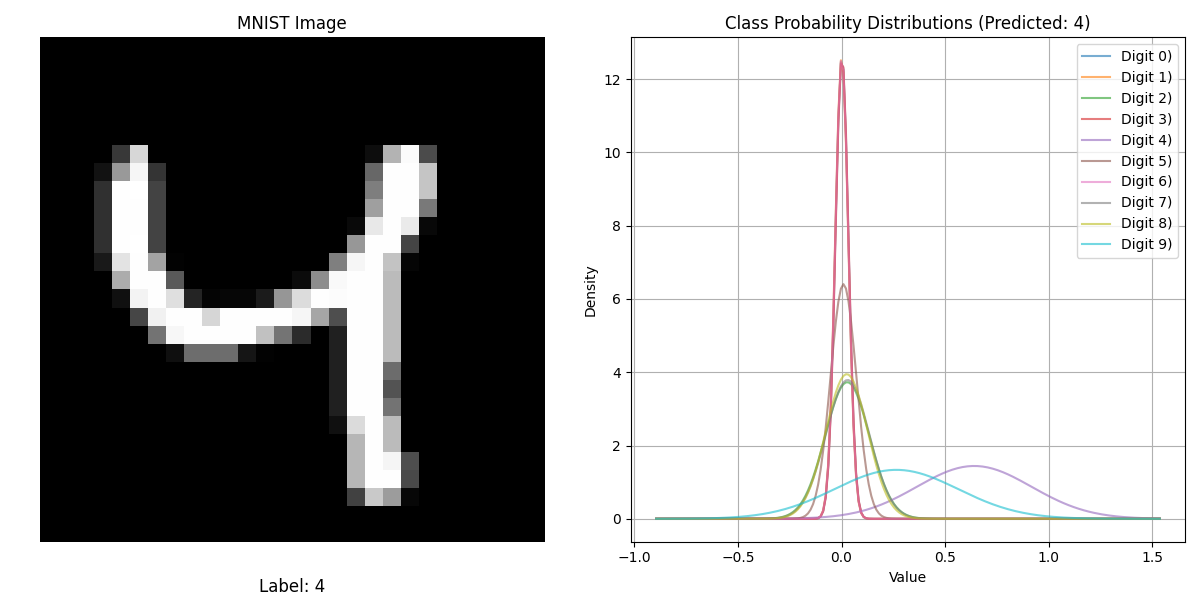
\includegraphics[width=1.0\linewidth]{Figures/4.png}
\caption{Ratio of predictions and epistemic uncertainty associated to each class on a MNIST \textit{4} image.}
\label{fig:remax_4}
\end{figure}


\begin{figure}[h]
\centering
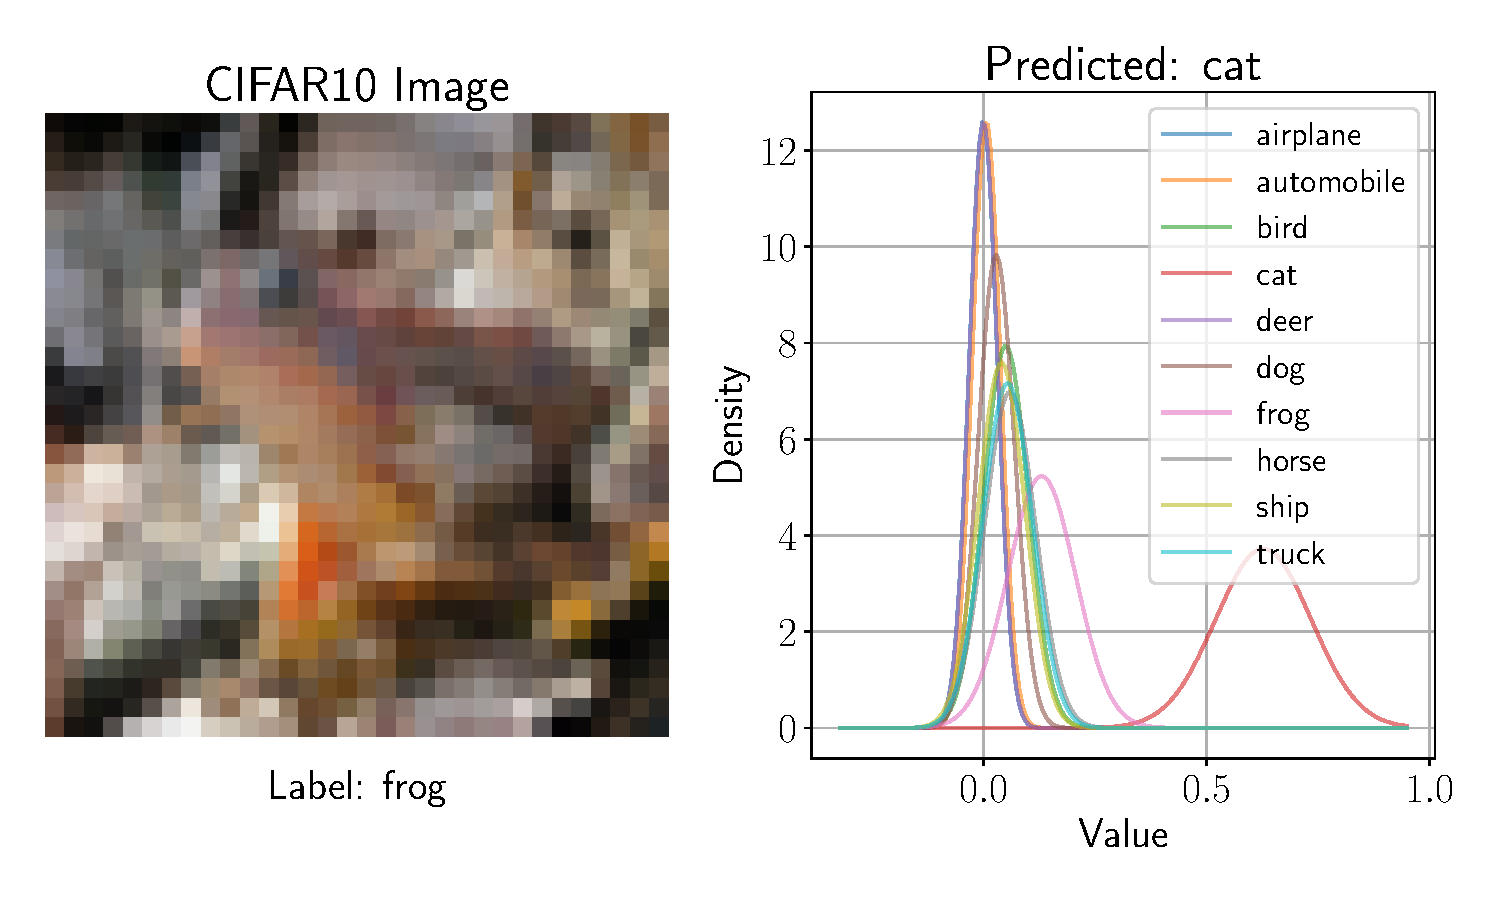
\includegraphics[width=1.0\linewidth]{Figures/frog.pdf}
\caption{Ratio of predictions and epistemic uncertainty associated to each class on a CIFAR10 \textit{frog} image.}
\label{fig:remax_frog}
\end{figure}


Figures \ref{fig:remax_4} and \ref{fig:remax_frog} illustrate the utility of the Remax activation function in classification tasks. In Figure \ref{fig:remax_4}, the class probabilities are represented by the means of Gaussian distributions, and the epistemic uncertainty—stemming from the model’s lack of knowledge due to insufficient data—is captured by the standard deviations. In Figure \ref{fig:remax_frog}, a misclassification example is shown where a frog is incorrectly predicted as a cat. However, the second most probable class is correctly identified as a frog, with both classes exhibiting considerable epistemic uncertainty. These examples highlight how Remax not only provides probabilistic predictions but also quantifies the model’s uncertainty.


\section{Comparative Analysis: TAGI vs. Torch}\label{sec:tagi_vs_torch}

In this section, we present a comprehensive comparison between the Tractable Approximate Gaussian Inference (TAGI) framework and a standard Torch-based backpropagation approach. Our analysis focuses on various aspects including overall performance, the impact of batch size, network depth, network size, the effect of the parameter $\sigma_v$ on TAGI, and training time considerations. We highlight key findings using a combination of summary tables and selected figures. In addition, we incorporate results from our new TAGI-Remax implementation. While it often converged reliably and performed similarly on average to TAGI-HRC, it rarely achieved the absolute lowest error rates across experiments, suggesting that its stability does not always translate into peak performance.

\subsection{Overall Performance}
Across all experiments, TAGI consistently demonstrated better average performance in terms of test error compared to Torch. This advantage is most pronounced when increasing the number of layers in the network. While Torch-based models struggled to converge or exhibited deteriorated performance with deeper networks (particularly in convolutional neural networks without batch normalization), TAGI maintained relatively stable error rates. This robustness suggests that TAGI may be less sensitive to architectural complexities and can effectively handle deeper networks without requiring additional normalization techniques.

The TAGI-Remax implementation followed a similar trend to TAGI-HRC in terms of average performance. As shown in Table~\ref{tab:overall_performance}, it also outperformed Torch in terms of test error. Although TAGI-Remax generally converged well, it did not frequently yield the absolute best results, indicating that while it is stable, it may not always produce the lowest achievable error.

% Overall Average Performance
\begin{table}[h]
\centering
\caption{Overall Average Training and Test Error Rates (\%) across Frameworks}
\label{tab:overall_performance}
\begin{small}
\begin{tabular}{lcc}
\toprule
Framework & Avg. Training Error & Avg. Test Error \\
\midrule
Torch      & 10.05 & 10.69 \\
TAGI-HRC   & 7.07  & \textbf{7.73}  \\
TAGI-Remax & 7.14  & \textbf{7.78}  \\
\bottomrule
\end{tabular}
\end{small}
\end{table}

The best overall performance was achieved by TAGI-HRC CNNs with three layers, 32 channels, and a sigma value of 0.5. Notably, the top experiments consistently featured TAGI-HRC CNNs rather than CNNs with batch normalization, highlighting TAGI's capability to deliver superior results without relying on normalization techniques. TAGI-Remax also benefited from similar settings, although it did not surpass the best TAGI-HRC configurations.

\subsection{Effect of Batch Size}
We observed a clear divergence in how each framework responds to varying batch sizes. Torch-based models tended to perform better with larger batch sizes, often relying on more stable gradient estimates to train effectively. Conversely, TAGI excelled with smaller batch sizes, where it could achieve remarkably low test errors even as network depth increased. This pattern is particularly striking in CNNs without batch normalization layers, where Torch's performance with smaller batch sizes was notably poor, while TAGI thrived under such conditions.

Interestingly, TAGI-Remax differed slightly from TAGI-HRC in terms of batch size sensitivity. While TAGI-HRC performed best with smaller batch sizes, TAGI-Remax appeared more flexible, showing stable performance across a range of batch sizes without a strong preference toward smaller batches.

% Impact of Batch Size
\begin{table}[h]
\centering
\caption{Test Error Rates (\%) by Batch Size and Framework (FNN and CNN only)}
\label{tab:batch_size_impact}
\begin{small}
\begin{tabular}{lcccc}
\toprule
 & \multicolumn{2}{c}{Small Batch (16)} & \multicolumn{2}{c}{Large Batch (512)} \\
Framework & FNN & CNN & FNN & CNN \\
\midrule
Torch      &  9.31 & 31.20 &  \textbf{5.03} & 16.22 \\
TAGI-HRC   & 10.42 & \textbf{1.74} & 12.14 & 15.99 \\
TAGI-Remax &  9.14 &  7.30 &  7.02 &  5.43 \\
\bottomrule
\end{tabular}
\end{small}
\end{table}

\subsection{Effect of Batch Normalization}
We explore here the impact of batch normalization and batch size on test error rates for both frameworks. Torch-based models exhibited superior performance in CNNs with batch normalization, particularly with larger batch sizes, where they achieved the lowest test error rates. In contrast, TAGI demonstrated remarkable consistency and robustness with smaller batch sizes, regardless of whether batch normalization was applied. Interestingly, in TAGI experiments, CNNs without batch normalization performed slightly better than their batch-normalized counterparts, highlighting that lower batch sizes are a more significant factor for TAGI's performance than applying batch normalization.

For TAGI-Remax, a similar pattern emerged. Batch normalization did not provide a clear advantage, and good performance often came from configurations without it. This parallels the original TAGI-HRC results, suggesting that both TAGI-HRC and TAGI-Remax benefit more from careful selection of batch sizes than from normalization techniques.

% Impact of Batch Normalization
\begin{table}[h]
\centering
\caption{Test Error Rates (\%) by Batch Size, Batch Normalization, and Framework (CNN only)}
\label{tab:batch_norm_batch_size_impact}
\begin{small}
\begin{tabular}{lcccc}
\toprule
 & \multicolumn{2}{c}{Small Batch (16)} & \multicolumn{2}{c}{Large Batch (512)} \\
Framework & With BN & W.o BN & With BN & W.o BN \\
\midrule
Torch      & \textbf{1.35} & 31.20 & \textbf{1.06} & 16.22 \\
TAGI-HRC   &  1.97         & \textbf{1.74} & 4.11 & 15.99 \\
TAGI-Remax & 12.05         &  7.30         & 5.75 &  5.43 \\
\bottomrule
\end{tabular}
\end{small}
\end{table}


\subsection{Influence of Network Depth}
Depth-sensitive behavior was a crucial point of differentiation. As the number of layers increased, Torch-based CNNs (without batch normalization) struggled to converge, resulting in significantly higher test errors. In contrast, TAGI-HRC remained relatively stable, offering effective training and lower test errors even with deeper architectures. This is a key finding, suggesting TAGI-HRC’s potential to alleviate the commonly observed training difficulties associated with very deep neural networks.

TAGI-Remax followed a similar trajectory to TAGI-HRC in this regard. While it did not consistently achieve the absolute lowest errors, it also did not succumb to the performance degradation seen with Torch models as the network depth increased. This indicates that the core resilience to depth-related training issues is preserved in the TAGI-Remax implementation.

% FIGURE: Test Error by Number of Layers
\begin{figure}[h]
\centering
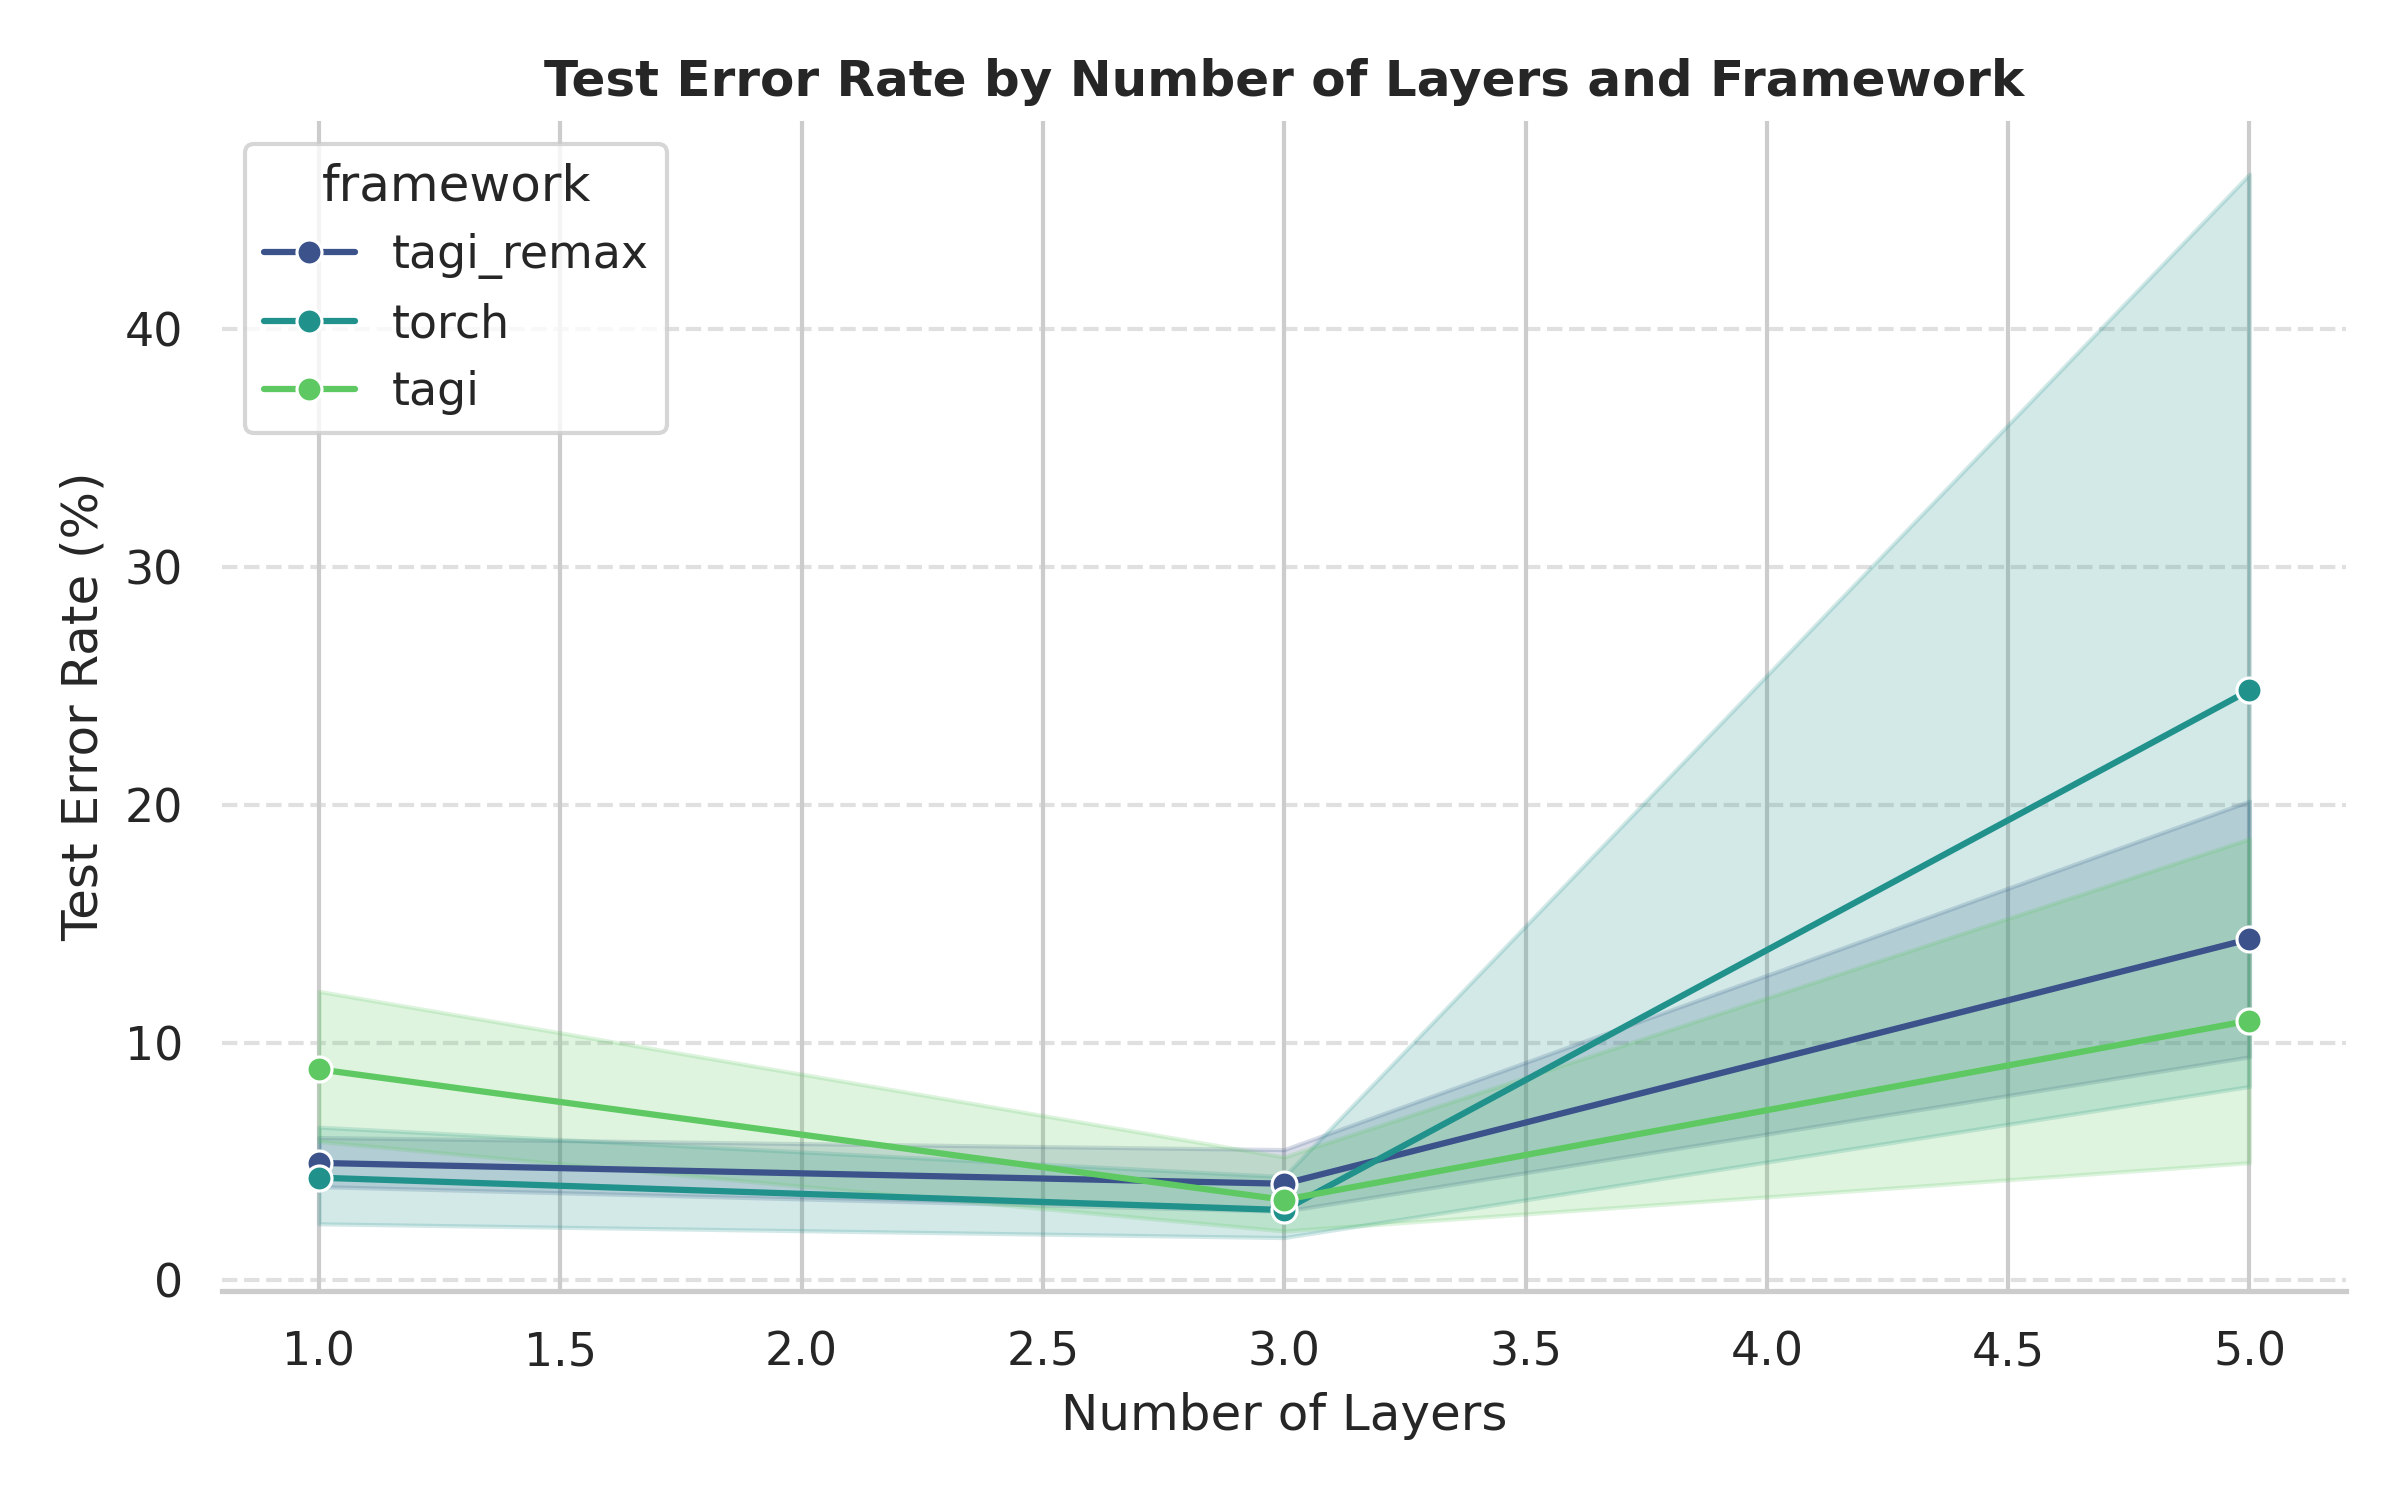
\includegraphics[width=1.0\linewidth]{Figures/num_layers_test_error.png}
\caption{Test Error Rate by Number of Layers for TAGI-HRC vs. Torch. TAGI-HRC maintains low error rates as depth increases, while Torch performance degrades significantly with deeper networks (especially CNNs without batch normalization).}
\label{fig:num_layers_comparison}
\end{figure}

\subsection{Effect of \texorpdfstring{$\sigma_v$}{sigma\_v} in TAGI}
The parameter $\sigma_v$ plays a pivotal role in TAGI’s performance. Our experiments indicate that higher values of $\sigma_v$ (e.g., $\sigma_v = 1.0$) yield better results, while a lower value (e.g., $\sigma_v = 0$) leads to poorer performance. This trend holds across different network depths, with deeper TAGI-HRC architectures benefiting even more from a larger $\sigma_v$. This finding underscores the importance of tuning $\sigma_v$ to enhance TAGI-HRC's representational capability and stability.

TAGI-Remax experiments mirrored these findings. The same upward trend in performance with increasing $\sigma_v$ values was observed, reinforcing the importance of this parameter for both implementations.

% FIGURE: TAGI Performance by sigma_v
\begin{figure}[h]
\centering
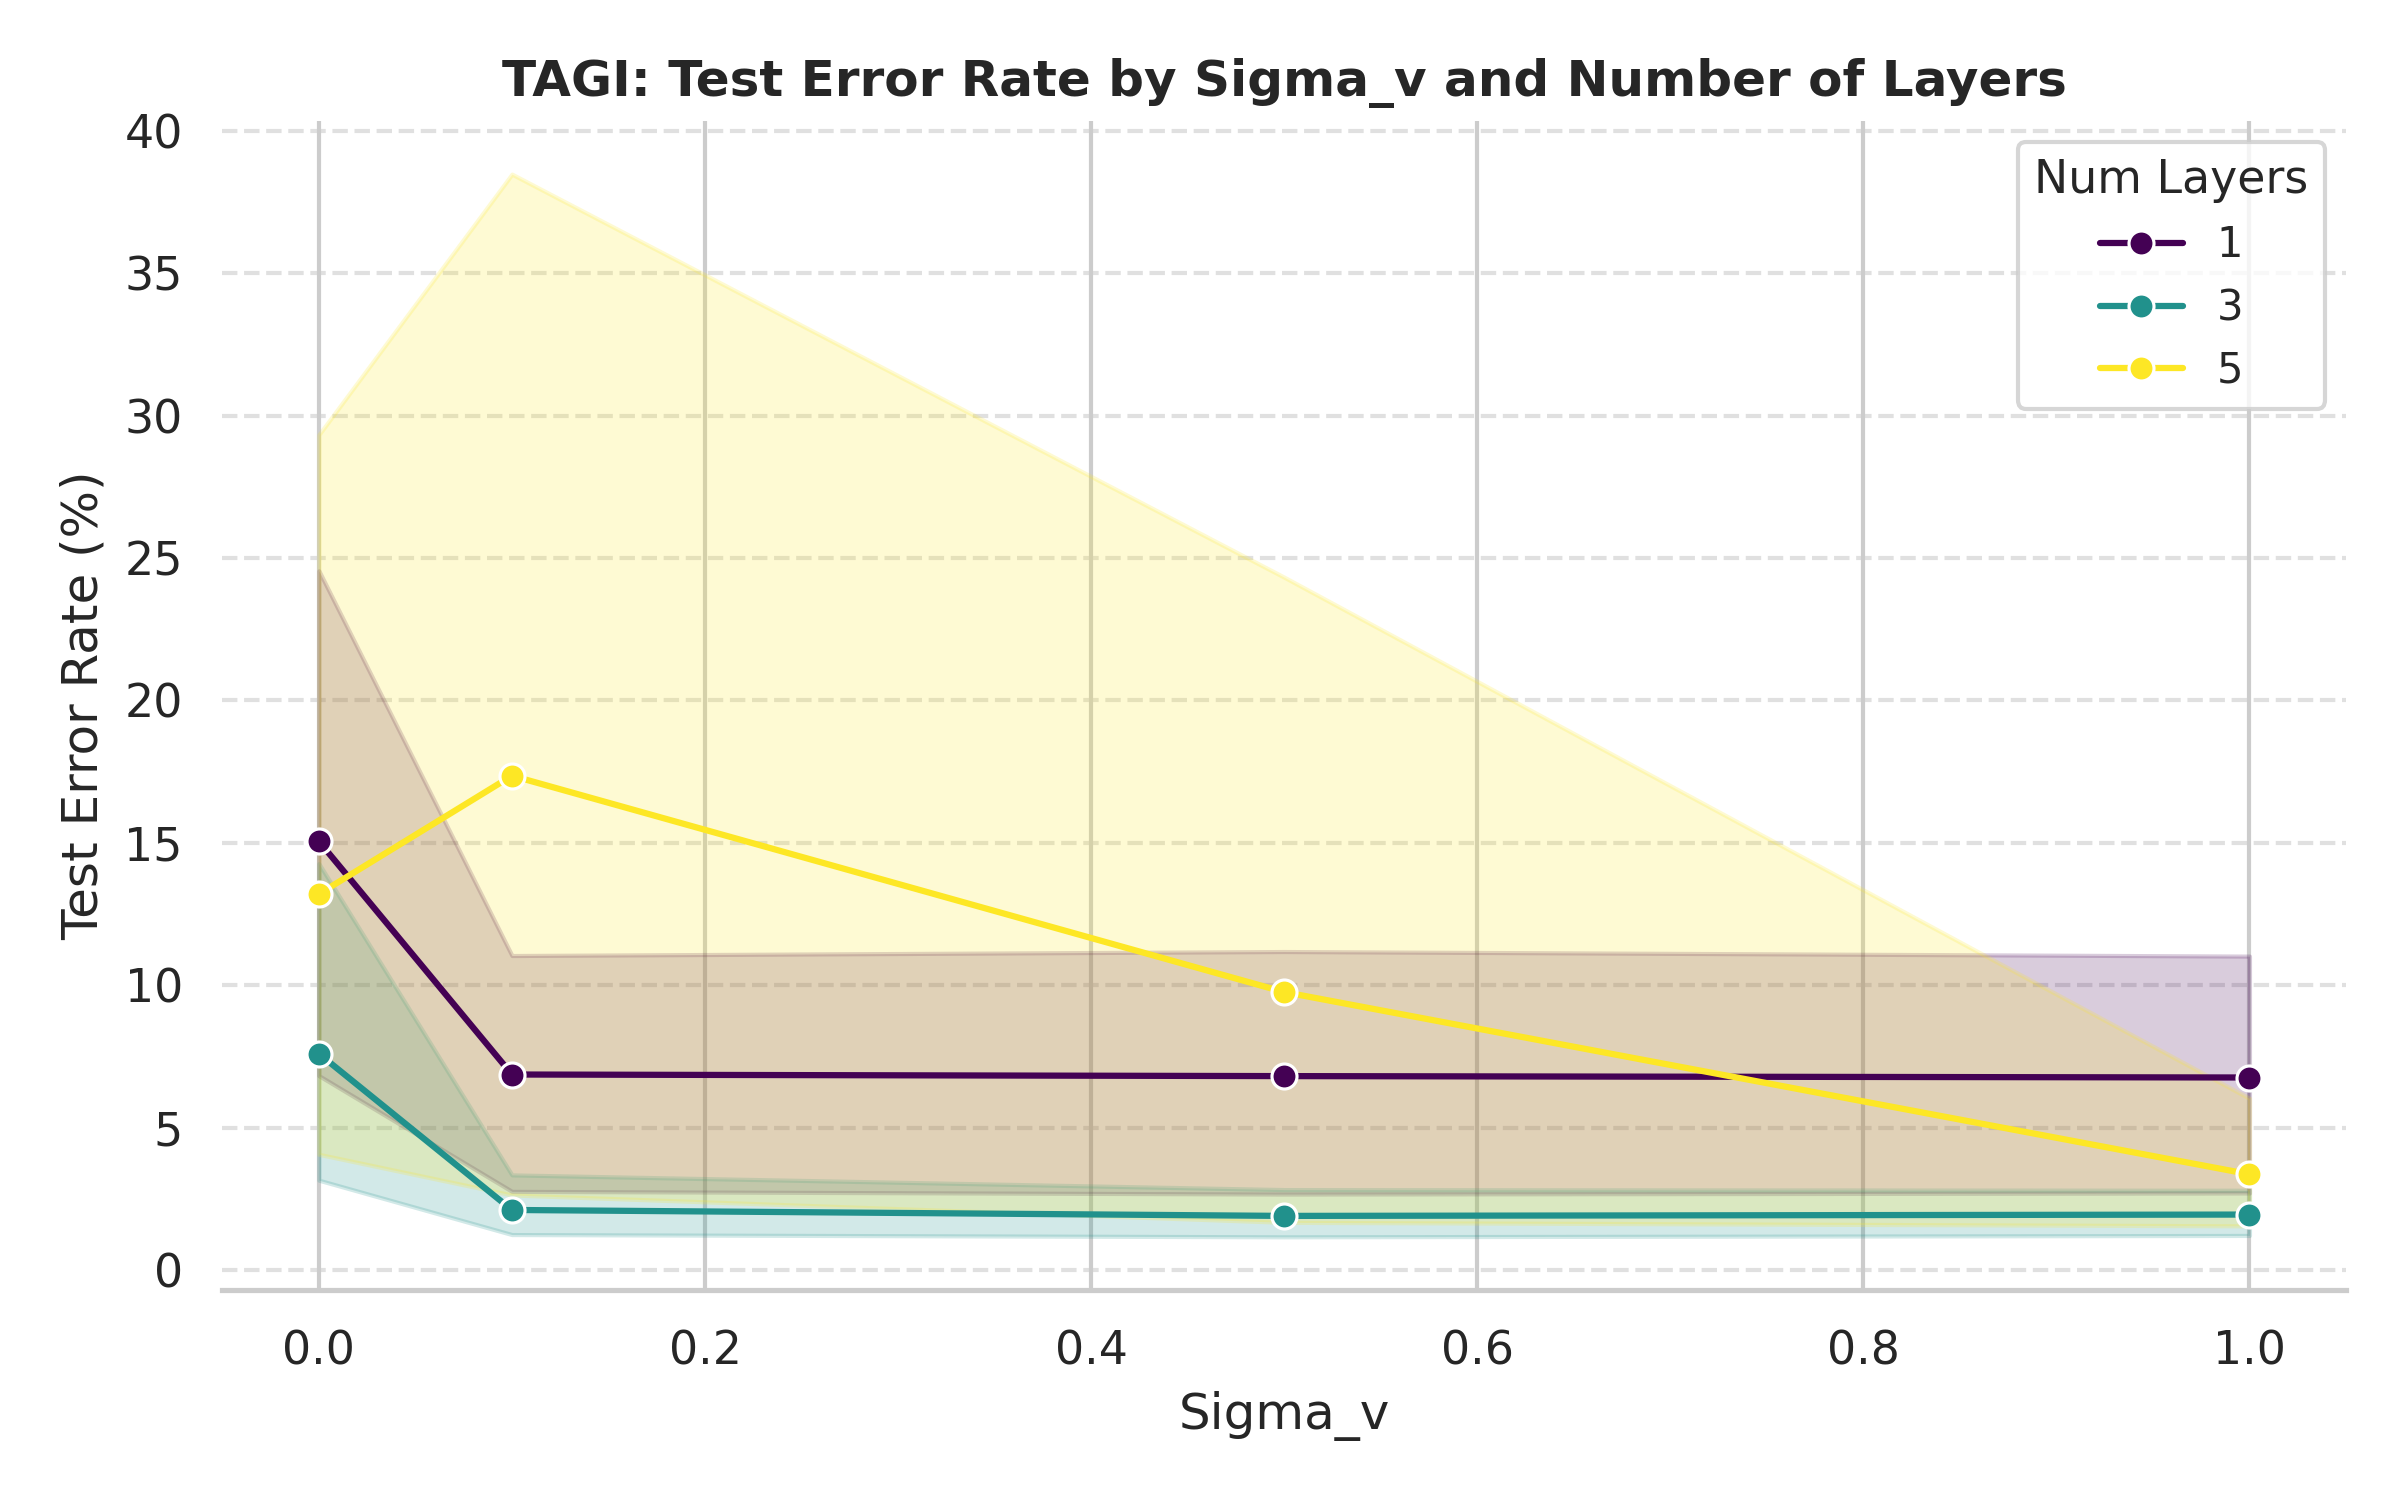
\includegraphics[width=1.0\linewidth]{Figures/tagi_sigma_comparison.png}
\caption{Impact of $\sigma_v$ on TAGI Performance across Different Network Depths. Higher $\sigma_v$ values consistently improve test error rates, especially in deeper networks.}
\label{fig:tagi_sigma}
\end{figure}

\subsection{Impact of Network Size (Neurons/Channels)}
In fully-connected neural networks (FNNs), increasing the number of neurons per layer benefited TAGI-HRC more than Torch. TAGI-HRC seemed to leverage the additional network capacity effectively, reducing test error as network width grew. By contrast, Torch did not show significant improvement when neurons per layer increased, suggesting a possible limitation in how it explores the representational capacity of larger networks. Similar trends were noted with CNNs when increasing the number of channels, reinforcing the notion that TAGI-HRC may inherently avoid overfitting and achieve better generalization with larger models.

TAGI-Remax followed a similar pattern in FNNs: increasing the number of neurons per layer led to better performance. However, in CNNs, increasing the number of channels did not improve results for TAGI-Remax and even led to worse performance. This discrepancy highlights that while TAGI-Remax retains many of the advantageous characteristics of TAGI-HRC, certain architectural expansions may not universally improve its outcomes.

% Impact of Network Size (Neurons per Layer)
\begin{table}[h]
\centering
\caption{FNN Test Error (\%) by Neurons per Layer (Averaged across Layers)}
\label{tab:fnn_neurons_impact}
\begin{small}
\begin{tabular}{lcc}
\toprule
 & Small (32) & Large (512) \\
Framework & Neurons/layer & Neurons/layer \\
\midrule
Torch      & 7.03 &  7.32 \\
TAGI-HRC   & 13.58         &  \textbf{8.98} \\
TAGI-Remax &  9.25         &  \textbf{6.91} \\
\bottomrule
\end{tabular}
\end{small}
\end{table}

% Impact of Network Size (Channels per Layer)
\begin{table}[h]
\centering
\caption{CNN Test Error (\%) by Initial Channels per Layer (Averaged)}
\label{tab:cnn_channels_impact}
\begin{small}
\begin{tabular}{lcc}
\toprule
 & Small (8) & Large (32) \\
Framework & Channels/layer & Channels/layer \\
\midrule
Torch      & 8.79 & 16.13 \\
TAGI-HRC   &  6.29         &  \textbf{5.61} \\
TAGI-Remax &  \textbf{5.46}         &  9.81 \\
\bottomrule
\end{tabular}
\end{small}
\end{table}

\subsection{Training Time Considerations}
While TAGI-HRC outperformed Torch in several qualitative aspects, it was generally more computationally expensive, especially as network depth increased. The training time for TAGI-HRC seemed to grow more rapidly than for Torch. In certain scenarios, Torch’s faster (but sometimes less effective) training made it a more practical choice, especially when architectural complexity was moderate and batch normalization was used to stabilize training. Also, Torch experiments with CNNs without batch normalization were stopped early, explaining the longer training time for three layers compared to five.

TAGI-Remax followed a similar trend. Although it often converged reliably, the computational overhead remained considerable. Its training time scaled in a manner similar to that of TAGI-HRC, suggesting that while stable and effective, both TAGI-HRC and TAGI-Remax incur higher computational costs than Torch as models grow in complexity.

% Training Time and Test Error by Number of Layers
\begin{table}[h]
\centering
\caption{Training Time (minutes) vs. Test Error (\%) by Number of Layers}
\label{tab:training_time}
\begin{small}
\begin{tabular}{lcccccc}
\toprule
Layers & \multicolumn{2}{c}{Torch} & \multicolumn{2}{c}{TAGI-HRC} & \multicolumn{2}{c}{TAGI-Remax} \\
 & Time & Err & Time & Err & Time & Err \\
\midrule
1 & 4.5 & 4.3 & 5.7 & 8.9 & 5.6 & 4.9 \\
3 & 5.6 & 3.0 & 6.6 & 3.4 & 6.5 & 4.1 \\
5 & 5.2 & 24.8 & \textbf{\textcolor{red}{16.4}} & 10.9 & \textbf{\textcolor{red}{13.0}} & 14.3 \\
\bottomrule
\end{tabular}
\end{small}
\end{table}

\subsection{Summary of Key Insights}
In summary, the TAGI framework provides a more robust learning mechanism across various dimensions—batch sizes, network depths, batch normalization, and network widths—resulting in lower test errors compared to Torch. However, these improvements often come at a higher computational cost. Additionally, the choice of $\sigma_v$ in TAGI can significantly influence performance, suggesting the importance of careful hyperparameter selection. Similarly, TAGI-Remax maintains these benefits and converges reliably, but does not consistently achieve the lowest possible error rates. It shares many of TAGI-HRC’s characteristics, including sensitivity to $\sigma_v$ and lower batch sizes, as well as improved performance with wider FNNs, but may not gain from wider CNNs. In contrast, Torch implementations benefit greatly from architectural and training heuristics like batch normalization and larger batch sizes, yet display notable limitations when confronted with deeper networks and smaller batch sizes.


% Acknowledgements should only appear in the accepted version.
\section*{Acknowledgements}

\textbf{Do not} include acknowledgements in the initial version of
the paper submitted for blind review.

If a paper is accepted, the final camera-ready version can (and
probably should) include acknowledgements. In this case, please
place such acknowledgements in an unnumbered section at the
end of the paper. Typically, this will include thanks to reviewers
who gave useful comments, to colleagues who contributed to the ideas,
and to funding agencies and corporate sponsors that provided financial
support.


% In the unusual situation where you want a paper to appear in the
% references without citing it in the main text, use \nocite
\nocite{langley00}

\bibliography{example_paper}
\bibliographystyle{icml2018}


%%%%%%%%%%%%%%%%%%%%%%%%%%%%%%%%%%%%%%%%%%%%%%%%%%%%%%%%%%%%%%%%%%%%%%%%%%%%%%%
%%%%%%%%%%%%%%%%%%%%%%%%%%%%%%%%%%%%%%%%%%%%%%%%%%%%%%%%%%%%%%%%%%%%%%%%%%%%%%%
% DELETE THIS PART. DO NOT PLACE CONTENT AFTER THE REFERENCES!
%%%%%%%%%%%%%%%%%%%%%%%%%%%%%%%%%%%%%%%%%%%%%%%%%%%%%%%%%%%%%%%%%%%%%%%%%%%%%%%
%%%%%%%%%%%%%%%%%%%%%%%%%%%%%%%%%%%%%%%%%%%%%%%%%%%%%%%%%%%%%%%%%%%%%%%%%%%%%%%
\appendix
\section{Do \emph{not} have an appendix here}

\textbf{\emph{Do not put content after the references.}}
%
Put anything that you might normally include after the references in a separate
supplementary file.

We recommend that you build supplementary material in a separate document.
If you must create one PDF and cut it up, please be careful to use a tool that
doesn't alter the margins, and that doesn't aggressively rewrite the PDF file.
pdftk usually works fine. 

\textbf{Please do not use Apple's preview to cut off supplementary material.} In
previous years it has altered margins, and created headaches at the camera-ready
stage. 
%%%%%%%%%%%%%%%%%%%%%%%%%%%%%%%%%%%%%%%%%%%%%%%%%%%%%%%%%%%%%%%%%%%%%%%%%%%%%%%
%%%%%%%%%%%%%%%%%%%%%%%%%%%%%%%%%%%%%%%%%%%%%%%%%%%%%%%%%%%%%%%%%%%%%%%%%%%%%%%


\end{document}


% This document was modified from the file originally made available by
% Pat Langley and Andrea Danyluk for ICML-2K. This version was created
% by Iain Murray in 2018. It was modified from a version from Dan Roy in
% 2017, which was based on a version from Lise Getoor and Tobias
% Scheffer, which was slightly modified from the 2010 version by
% Thorsten Joachims & Johannes Fuernkranz, slightly modified from the
% 2009 version by Kiri Wagstaff and Sam Roweis's 2008 version, which is
% slightly modified from Prasad Tadepalli's 2007 version which is a
% lightly changed version of the previous year's version by Andrew
% Moore, which was in turn edited from those of Kristian Kersting and
% Codrina Lauth. Alex Smola contributed to the algorithmic style files.
